\documentclass[a4paper,11pt]{article}
\usepackage[utf8]{inputenc}
\usepackage[T1]{fontenc}
\usepackage[french]{babel}
\usepackage{amsmath,amssymb}
\usepackage{geometry}
\usepackage{tikz}
\usepackage{enumitem}
\usepackage{fancyhdr}
\usepackage{tcolorbox}
\usepackage{pgfplots}
\pgfplotsset{compat=1.18}
\usepackage{graphicx}

\geometry{margin=2cm}
\setlength{\headheight}{14pt}

\pagestyle{fancy}
\fancyhf{}
\lhead{BTS -- Mathématiques}
\rhead{Devoir Maison -- Séries de Fourier}
\cfoot{\thepage}

\tcbset{
  exobox/.style={colback=orange!5!white, colframe=orange!60!black, fonttitle=\bfseries, title=#1},
  reponsebox/.style={colback=gray!5!white, colframe=gray!40!black, sharp corners, boxrule=0.5pt, left=4pt, right=4pt, top=4pt, bottom=4pt}
}

\newcommand{\dt}{\mathrm{d}t}

\begin{document}

\begin{center}
  {\LARGE \textbf{Devoir Maison -- Séries de Fourier}} \\[0.2cm]
  {\Large Calcul des coefficients $a_0$, $a_n$ et $b_n$} \\[0.2cm]
  \rule{0.6\textwidth}{0.4pt} \\[0.2cm]
  {\normalsize À rendre le : \dotfill \quad Calculatrice autorisée} \\[0.1cm]
  {\normalsize Le barème est donné à titre indicatif.}
\end{center}

\vspace{0.2cm}

\noindent\textbf{Nom :} \dotfill \quad \textbf{Prénom :} \dotfill \quad \textbf{Classe :} \dotfill

\vspace{0.3cm}

\noindent\fbox{\parbox{\dimexpr\textwidth-2\fboxsep-2\fboxrule}{%
\textbf{Rappels :} Soit $f$ une fonction périodique de période $T$ et de pulsation $\omega = \dfrac{2\pi}{T}$. Son développement en série de Fourier est :
\[
  S(t) = a_0 + \sum_{n=1}^{+\infty}\!\bigl(a_n\cos(n\omega t)+b_n\sin(n\omega t)\bigr)
\]
avec \quad
$\displaystyle a_0 = \frac{1}{T}\int_0^{T} f(t)\,\dt$,\qquad
$\displaystyle a_n = \frac{2}{T}\int_0^{T} f(t)\cos(n\omega t)\,\dt$,\qquad
$\displaystyle b_n = \frac{2}{T}\int_0^{T} f(t)\sin(n\omega t)\,\dt$.
}}

\vspace{0.4cm}

%% ================================================================
%% EXERCICE 1 — 10 points
%% ================================================================
\begin{tcolorbox}[exobox={Exercice 1 \hfill \normalfont\textit{(10 points)}}]
  On considère la fonction $f$ périodique de période $T = 2$, définie sur $[0\,;\,2[$ par :
  \[
    f(t) = \begin{cases} 4 & \text{si } 0 \leq t < 1 \\ 0 & \text{si } 1 \leq t < 2 \end{cases}
  \]
\end{tcolorbox}

\begin{center}
  \begin{tikzpicture}
    \begin{axis}[
      axis lines=middle,
      xlabel={$t$},
      ylabel={$f(t)$},
      xmin=-2.5, xmax=6.5,
      ymin=-0.5, ymax=5.5,
      xtick={-2,-1,0,1,2,3,4,5,6},
      ytick={0,1,2,3,4},
      width=13cm, height=4.5cm,
      grid=major,
      grid style={dashed, gray!30},
    ]
    \addplot[blue, ultra thick, domain=-2:-1] {4};
    \addplot[blue, ultra thick, domain=-1:0]  {0};
    \addplot[blue, ultra thick, domain=0:1]   {4};
    \addplot[blue, ultra thick, domain=1:2]   {0};
    \addplot[blue, ultra thick, domain=2:3]   {4};
    \addplot[blue, ultra thick, domain=3:4]   {0};
    \addplot[blue, ultra thick, domain=4:5]   {4};
    \addplot[blue, ultra thick, domain=5:6]   {0};
    \addplot[blue, dashed, thin] coordinates {(-1,4)(-1,0)};
    \addplot[blue, dashed, thin] coordinates {(1,4)(1,0)};
    \addplot[blue, dashed, thin] coordinates {(3,4)(3,0)};
    \addplot[blue, dashed, thin] coordinates {(5,4)(5,0)};
    \end{axis}
  \end{tikzpicture}
\end{center}

\begin{enumerate}[label=\textbf{\arabic*.}]
  \item Donner la valeur de la pulsation $\omega$. \hfill \textit{(1 pt)}
  \begin{tcolorbox}[reponsebox, height=1.3cm]\end{tcolorbox}

  \item Calculer $a_0$. \hfill \textit{(2 pts)}
  \begin{tcolorbox}[reponsebox, height=1.5cm]\end{tcolorbox}

  \item Calculer $a_n$ pour tout entier $n \geq 1$.
        Que peut-on dire de tous les coefficients $a_n$ ? \hfill \textit{(2 pts)}
  \begin{tcolorbox}[reponsebox, height=3.5cm]\end{tcolorbox}

  \item Calculer $b_n$ pour tout entier $n \geq 1$.
        En déduire les valeurs exactes de $b_1$, $b_2$ et $b_3$. \hfill \textit{(4 pts)}
  \begin{tcolorbox}[reponsebox, height=5.5cm]\end{tcolorbox}

  \item Écrire le développement en série de Fourier $S(t)$ jusqu'à $n = 3$. \hfill \textit{(1 pt)}
  \begin{tcolorbox}[reponsebox, height=2cm]\end{tcolorbox}
\end{enumerate}

\vspace{3cm}

%% ================================================================
%% EXERCICE 2 — 10 points
%% ================================================================
\begin{tcolorbox}[exobox={Exercice 2 \hfill \normalfont\textit{(10 points)}}]
  On considère la fonction $f$ périodique de période $T = 4$, définie sur $[0\,;\,4[$ par :
  \[
    f(t) = \begin{cases} 3 & \text{si } 0 \leq t < 1 \\ 0 & \text{si } 1 \leq t < 4 \end{cases}
  \]
\end{tcolorbox}

\begin{enumerate}[label=\textbf{\arabic*.}]
  \item Tracer le signal $f$ sur $[-4\,;\,8]$ dans le repère ci-dessous. \hfill \textit{(1,5 pts)}

  \begin{center}
    \begin{tikzpicture}
      \begin{axis}[
        axis lines=middle,
        xlabel={$t$},
        ylabel={$f(t)$},
        xmin=-4.5, xmax=8.5,
        ymin=-0.4, ymax=4.2,
        xtick={-4,-3,-2,-1,0,1,2,3,4,5,6,7,8},
        ytick={0,1,2,3},
        width=14cm, height=4.8cm,
        grid=major,
        grid style={dashed, gray!30},
      ]
      \end{axis}
    \end{tikzpicture}
  \end{center}

  \item Donner la valeur de la pulsation $\omega$. \hfill \textit{(0,5 pt)}
  \begin{tcolorbox}[reponsebox, height=1.2cm]\end{tcolorbox}

  \item Calculer $a_0$. \hfill \textit{(2 pts)}
  \begin{tcolorbox}[reponsebox, height=1.5cm]\end{tcolorbox}

  \item Calculer $a_n$ pour tout entier $n \geq 1$.
        En déduire les valeurs exactes de $a_1$, $a_2$ et $a_3$. \hfill \textit{(3 pts)}
  \begin{tcolorbox}[reponsebox, height=5cm]\end{tcolorbox}
  
  

  \item Calculer $b_n$ pour tout entier $n \geq 1$.
        En déduire les valeurs exactes de $b_1$, $b_2$ et $b_3$. \hfill \textit{(3 pts)}
  \begin{tcolorbox}[reponsebox, height=5cm]\end{tcolorbox}
  
    \item Écrire le développement en série de Fourier $S(t)$ jusqu'à $n = 3$. \hfill \textit{(1 pt)}
  \begin{tcolorbox}[reponsebox, height=2cm]\end{tcolorbox}


\end{enumerate}

\newpage

%% ================================================================
%% BONUS — Tracé de S4
%% ================================================================
\begin{tcolorbox}[exobox={Bonus -- Illustration graphique}]
  On donne ci-dessous le tracé de la somme partielle obtenue à partir de l'exercice~2 :
  \[
    S_4(x) = \frac{1}{4} + \frac{1}{\pi}\cos x + \frac{1}{\pi}\sin x
             + \frac{1}{\pi}\sin 2x - \frac{1}{3\pi}\cos 3x + \frac{1}{3\pi}\sin 3x
  \]
\end{tcolorbox}

\vspace{0.3cm}

\begin{center}
  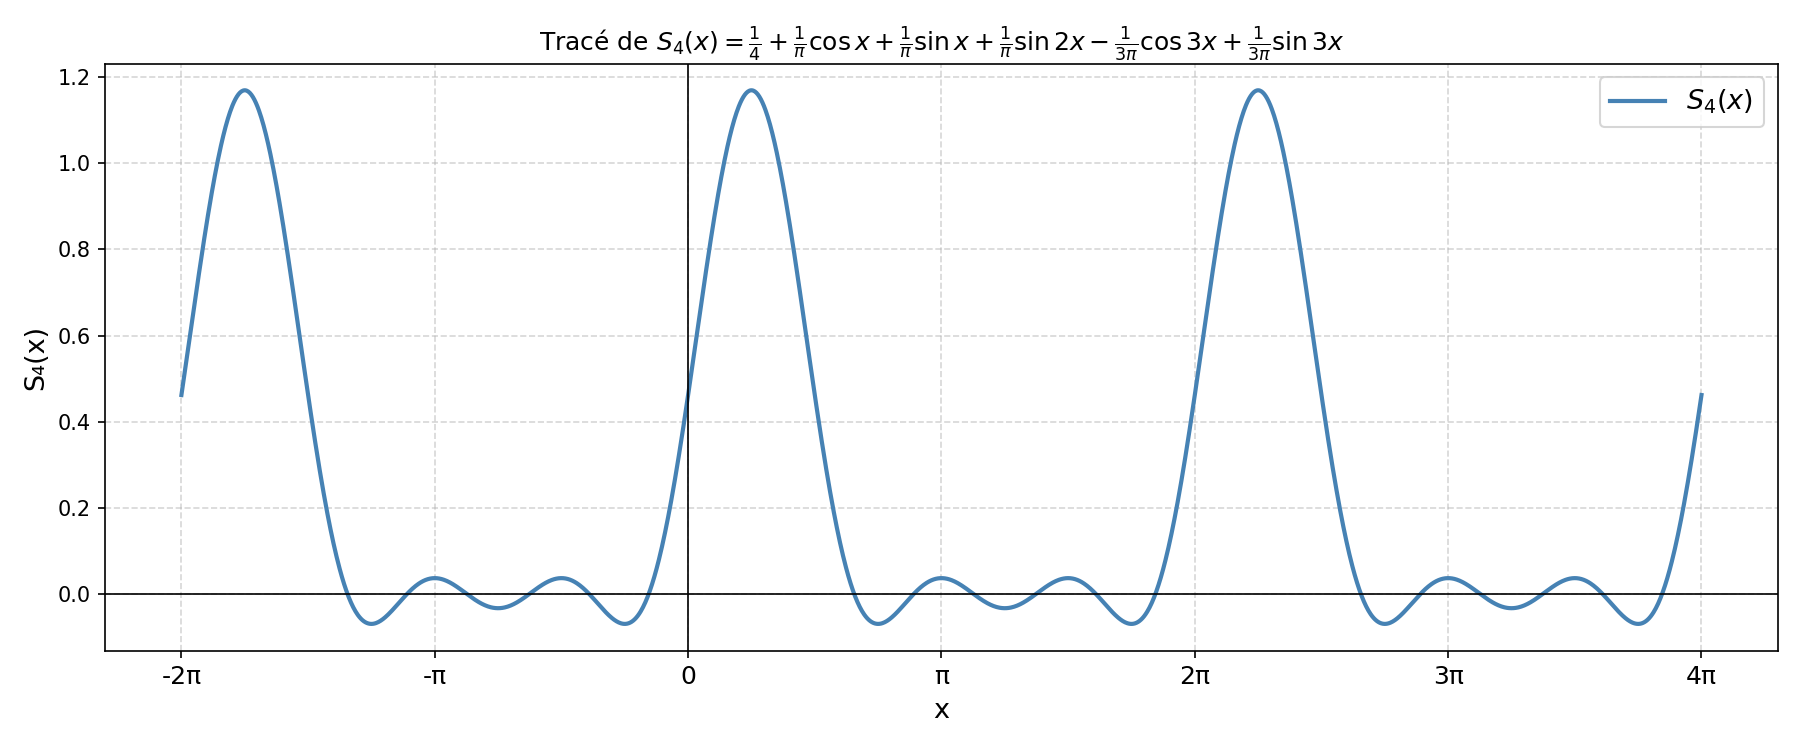
\includegraphics[width=\linewidth]{S4_fourier.png}
\end{center}

\vspace{0.2cm}

\noindent Commenter l'allure de la courbe : vers quelle fonction $f$ semble-t-elle converger au fur et à mesure que l'on ajoute des harmoniques ?

\begin{tcolorbox}[reponsebox, height=2.5cm]\end{tcolorbox}

\end{document}
